\subsection{题目描述}
Electron in the finite square-well potential is, \( (V_0 = 10 \, \text{eV}, \, a = 0.2 \, \text{nm}) \)

\begin{figure}[h!]
    \centering
    \begin{minipage}{0.45\textwidth}
        \[
            V(x) =
            \begin{cases}
                V_0 & x \leq -a \quad \text{Region I}   \\
                0   & -a < x < a \quad \text{Region II} \\
                V_0 & x \geq a \quad \text{Region III}
            \end{cases}
        \]
    \end{minipage}
    \hspace{0.05\textwidth} % 控制间距
    \begin{minipage}{0.4\textwidth}
        \centering
        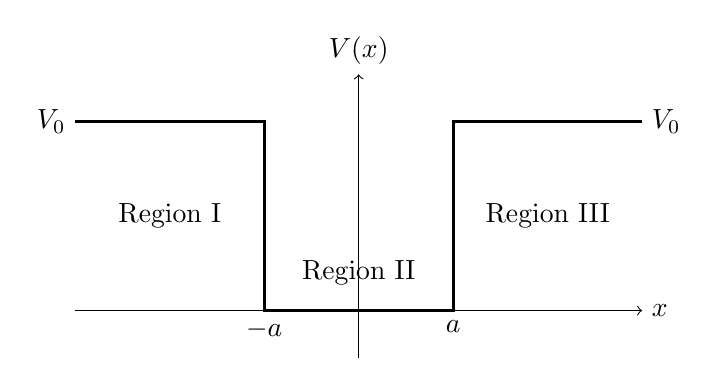
\begin{tikzpicture}[scale=1.2] % 缩放值按需调整
            % Potential well
            \draw[very thick] (-3,2) -- (-1,2) -- (-1,0) -- (1,0) -- (1,2) -- (3,2);
            \draw[->] (-3,0) -- (3,0) node[right] {$x$};
            \draw[->] (0,-0.5) -- (0,2.5) node[above] {$V(x)$};

            % Labels
            \node at (-2, 1) {Region I};
            \node at (0, 0.4) {Region II};
            \node at (2, 1) {Region III};

            \node[left] at (-3, 2) {$V_0$};
            \node[right] at (3, 2) {$V_0$};

            \node[below] at (-1,0) {$-a$};
            \node[below] at (1,0) {$a$};
        \end{tikzpicture}
    \end{minipage}
    \caption{Finite square-well potential and its corresponding mathematical expression.}
\end{figure}


Find the three lowest eigen states (\textbf{both} energies and wavefunctions).
\subsection{程序描述}
两种算法,一种针对本题的解析求解,即超越方程图解法:\texttt{./Codes/Problem 3/potential.py},另一种是数值求解:\texttt{./Codes/Problem 3/schrodinger.py},差分表示哈密顿矩阵,适用于更广泛的势能,偷懒都用Python实现了。
\subsection{伪代码}


\subsection{结果示例}
\begin{figure}[H]
    \centering
    \includegraphics[width=1.0\textwidth]{Figs/3_fun.png}
    \caption{\texttt{potential.py}解析图解法}
    \label{fig:3_py_fun}
\end{figure}

\begin{figure}[H]
    \centering
    \includegraphics[width=1.0\textwidth]{Figs/3_diff.png}
    \caption{\texttt{schrodinger.py}数值差分法}
    \label{fig:3_py_diff}
\end{figure}